\documentclass[]{article}



\usepackage{graphicx,forloop,caption,subcaption,float,hyperref,arrayjob,listings,color,booktabs,mathtools}
\usepackage{pdfpages}
\usepackage[margin=1.2in]{geometry}
\usepackage{amsmath}
\usepackage{multirow}
%vhdl code
\definecolor{dkgreen}{rgb}{0,0.6,0}
\definecolor{gray}{rgb}{0.5,0.5,0.5}
\definecolor{mauve}{rgb}{0.58,0,0.82}

\DeclareMathOperator*{\argmin}{\arg\!\min}
\newcommand{\rom}[1]{\uppercase\expandafter{\romannumeral#1}}

\lstset{frame=tb,
  language=VHDL,
  aboveskip=3mm,
  belowskip=3mm,
  showstringspaces=false,
  columns=flexible,
  basicstyle={\small\ttfamily},
  numbers=none,
  numberstyle=\tiny\color{gray},
  keywordstyle=\color{blue},
  commentstyle=\color{dkgreen},
  stringstyle=\color{mauve},
  breaklines=true,
  breakatwhitespace=true
  tabsize=3
}

%matlab code
\lstset{frame=tb,
  language=Matlab,
  aboveskip=3mm,
  belowskip=3mm,
  showstringspaces=false,
  columns=flexible,
  basicstyle={\small\ttfamily},
  numbers=none,
  numberstyle=\tiny\color{gray},
  keywordstyle=\color{blue},
  commentstyle=\color{dkgreen},
  stringstyle=\color{mauve},
  breaklines=true,
  breakatwhitespace=true
  tabsize=3
}


% Title Page
\title{UCLA\\EE230B\\Digital Communication Design Project\\Step 4 Report}
\author{Alican Salor 404271991 \\  \href{mailto:alicansalor@ucla.edu}{alicansalor@ucla.edu} \\ \\
Darren Reis 804359840 \\
\href{mailto:darrer.r.reis@gmail.com}{darren.r.reis@gmail.com} }


\begin{document}
\maketitle

\newpage
\tableofcontents

\newpage

\section{Background}
\label{sec:background}
This step of the project introduces complications from using computers and digital methods to analyze analog signals.  Data conversion can lead to additional, even catastrophic errors.\\
Recall, digital signals are quantized into samples, discrete points in time.  Conversely, an analog signal has a continuous value.  Going from one to the other requires a converter.  To take an analog signal and digitize it, an Analog-to-Digial Converter (A/D) is used.  Both types of signals are shown in Figure~\ref{fig:digitization}.  There is a wrinkle: the rate of conversion is critical to preserving the information.  By the Nyquist-Shannon Sampling Theorem (\ref{eq:nyquist}), the sampling frequency must be at least twice the highest frequency in the signal.  Without 
reaching this frequency, the samples can wrongfully convey a lower frequency signal, alias, of the true signal.  This is shown in Figure~\ref{fig:alias}.  

\begin{align}
\label{eq:nyquist}
f_s \geq 2 f_{max}
\end{align}


\begin{figure}[h]
        \centering
        \begin{subfigure}[b]{0.4\textwidth}
                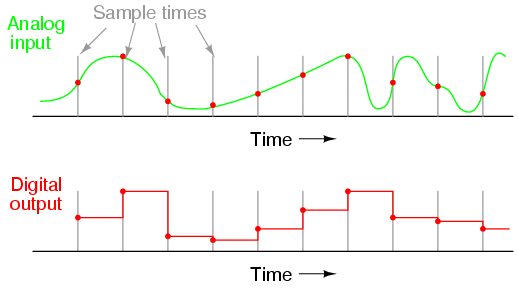
\includegraphics[width=\textwidth]{digitization.png}
                \caption{Analog and Digital signals}
                \label{fig:digitization}
        \end{subfigure}%
        \qquad \quad %add desired spacing between images, e. g. ~, \quad, \qquad etc.
          %(or a blank line to force the subfigure onto a new line)
        \begin{subfigure}[b]{0.5\textwidth}
                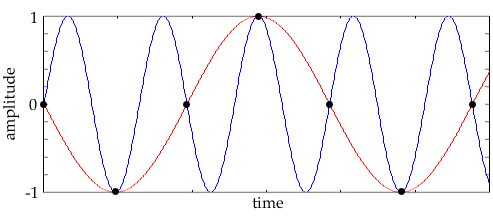
\includegraphics[width=\textwidth]{aliasing.jpg}
                \caption{Aliasing \label{fig:alias} \cite{aliasing}}
                \label{fig:alias}
        \end{subfigure}
        \caption{Digital Conversion \label{fig:digitize}}
\end{figure}

\begin{figure}[H]
\centering
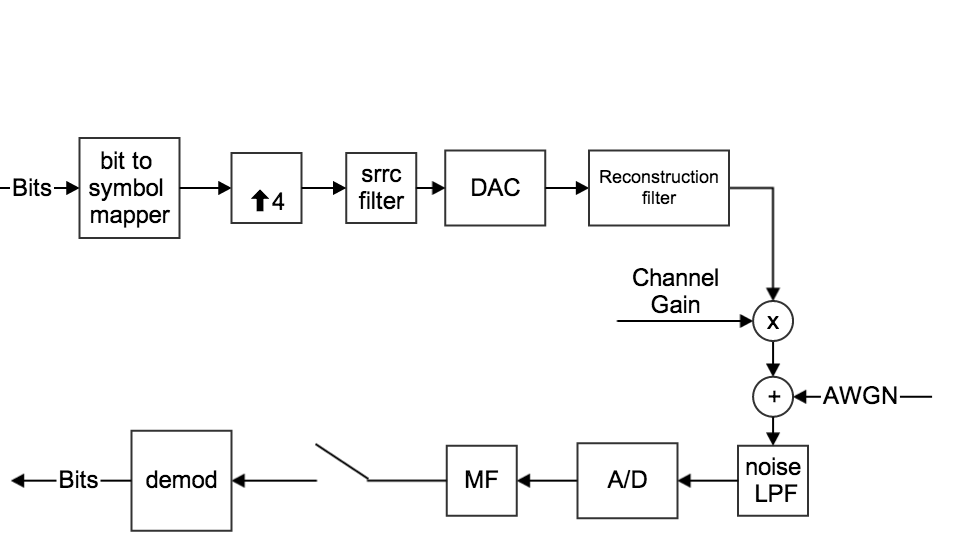
\includegraphics[width=0.5\textwidth]{step4.png}
\caption{Block Diagram of Step 4 system setup }
\end{figure}

\section{System}
\label{sec:system}
The system simulation model is shown in Figure~\ref{fig:step4}.  As from Step 1, bits are converted into symbols and then upsampled by adding in zeros.  This then is run through a Square Root Raised Cosine (SRRC) pulse shape filter.  This shaping improves the resistance of the sequence to intersymbol interference (ISI).  The output of this filter is fed into a Digital-to-Analog Converter (DAC).  A DAC takes the digital samples and zero-order holds them at a constant voltage, creating an analog signal.  \\
In our model, we then use a filter to restrict the bandwidth of the signals and facilitate transmission.  After the digitizer, a reconstruction filter (also sometimes called an anti-imaging filter) bandlimits the analog waveform output from the DAC.  The high frequency content contained in the stair-case digital signal is undesirable since it can create aliasing of wrongfully high frequency waves.  To avoid this, a Low Pass Filter is used for the reconstruction.  Ours is modeled as BUTTERWORTH.  BECAUSE BLAH BLAH.  This analog signal is then sent through a real world channel, modeled by gain and additive white Gaussian noise.  \\
To bring the analog back to the digital world, an A/D will be used.  However, just like before, the conversion can be improved by the use of a filter.  An anti-aliasing low-pass filter can constrain, or band limit, the channel noise before entering the A/D.  In this setting, the LPF  protects against aliasing of high frequency content being recorded at the lower frequency.\\
The end of the simulation model is identical to the process in Step 1: a matched filter to the SRRC picks out the symbols from the noisy received signal.  Afterwards, a sampler recovers the symbols before a demodulator converts the symbols back into bits.  

\begin{figure}[H]
\centering
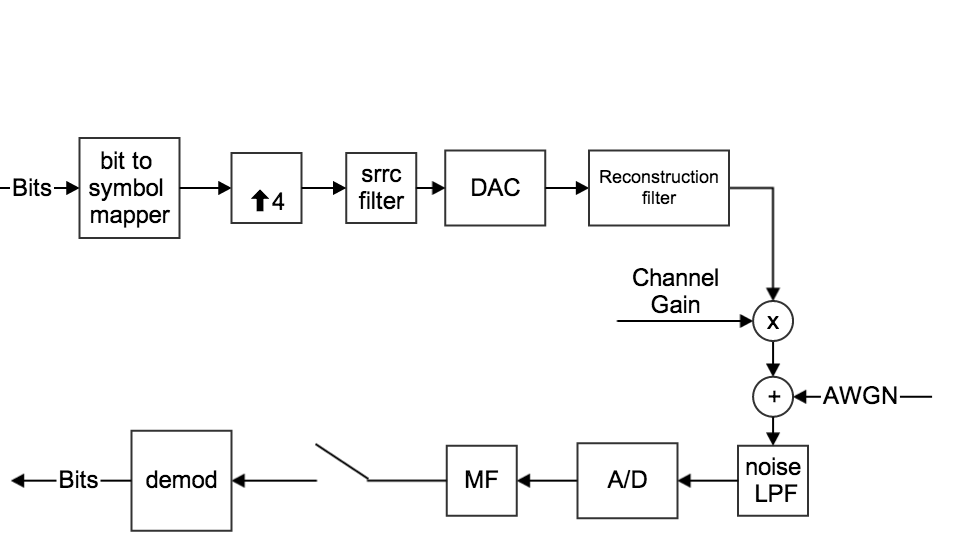
\includegraphics[width=\textwidth]{step4.png}
\caption{Block Diagram of Step 4 system setup\label{fig:step4}}
\end{figure}


To handle the noncoherent error introduced into the system, feedback loops (Costas and Decision Directed) were installed.  As from before, the $\delta\phi$ block represents a block that introduces phase or frequency offset on the carrier.  To combat this, the error is estimated and then fed into a feedback loop filter to track it out. \\

Both of these setups are based on the same control theory fundamentals and thus have similar feedback loop components. In control theory when there is steady state error in the open loop system, feedback, or `closing the loop' can track out the error.  From the plots in Step 2, we realize our situation is just this case of steady state error.  Depending on the order of the system, this error can become unbounded and damning.  Feedback can track or bound this error by `closing the loop' if the open loop system Type is 0.  \footnote{Recall, a system is of Type N when there are N poles at the s-plane origin.}  Here, the steady state error can be held to a certain level by introducing integration in the feedback line of the loop.  For us, this is true when we talk about phase error: we can send a step input phase error into a Voltage Controlled Oscillator and watch the error converge to a constant level. 
\begin{align}
\label{eq:vco}
\phi_{\text{out}} &= \int \! k_{VCO}V_{in} \mathrm{d}t
\end{align}
A VCO is a device with output oscillation which is varied by the voltage level of the input.  The transfer function, relating the input to the output, for this block is shown in Equation~\ref{eq:vco}. The integral action can eliminate phase error, as we see in Figure~\ref{fig:BLAH}.  To implement a VCO in simulation, a phase accumulator does the integration   action and then, to keep the result in the correct domain, the result is put through a modulo $2\pi$ block.   
When the plant is of higher Type than 0, as with a frequency offset, the steady state error can grow unbounded.  To deal with this scenario, another block is inserted in the feedback line.  An additional integrator increases the order of the closed loop system to allow bounding of higher type systems.  Notice in Figure~\ref{fig:costas}, the loop filter is Proportional-Integral.  With two integrators in the feedback path, Type 1 systems, or those with ramp inputs, can be bounded to a constant steady state error level.  Because frequency can be thought of as first order phase [\ref{eq:phaseFreq}], we track out the frequency error.\\
\begin{align}
\label{eq:phaseFreq}
\phi &= \int \! 2\pi f \mathrm{d}t 
\end{align}


Furthermore, as  can be seen in the simulation files, a different approach of coding is taken compared to the previous simulations. Note that unlike in previous simulations of the system, this analysis required sample-wise operations instead of signal-wise operations. That is, to maintain causality, the samples were analyzed one by one so that future samples could not influence present values.\\

In the following sections, the two setups for error recovery are given and their error metrics are examined.


\newpage

\subsection{System with Costas Loop}
This error recovery is accomplished first via a Costas loop, as in Figure~\ref{fig:costas}. 


The phase and frequency offset error, under QPSK, can be handled by the Costas loop given above. The technique first creates an estimate of the phase error by creating a metric for it.  The error is then sent through a closed feedback loop.  This structure can track out the zero order (phase offset) and first order (carrier offset) phase errors as it contains two integrators. 

In a Costas loop, the I and Q component of the received signal are both sent through a $\tanh\left(\cdot\right)$ block in order to discern their sign.  This works because, for $k>>1$, $\text{sign}\left(x\right) \approx \tanh \left(x\right)$.  These $\pm1$ signals are multiplied by the opposite component signal.  The I component is then subtracted from the Q component, creating a phase error metric [\ref{eq:costas}].  This is labeled in Figure~\ref{fig:costas} as \rom{1}. 

\begin{align}
  \label{eq:costas}
  S_{\rom{1}} &= \left[I\left(t\right)\sin\left(\phi_e\right)+Q\left(t\right)\cos\left(\phi_e\right)\right]\text{sign}\left(I\left(t\right)\cos\left(\phi_e\right)- Q\left(t\right)\sin\left(\phi_e\right)\right)\nonumber \\
  &\qquad {} - \left[I\left(t\right)\cos\left(\phi_e\right)-Q\left(t\right)\sin\left(\phi_e\right)\right]\text{sign}\left(I\left(t\right)\sin\left(\phi_e\right)+Q\left(t\right)\cos\left(\phi_e\right)\right)
  \end{align}


Equation~\ref{eq:costas} is the metric for phase error.  This value is run into the loop filter and then the VCO.  Finally, the output of the VCO is used to correct the received signal's phase error as seen in the system setup in Figure~\ref{fig:costas}.

\newpage
\section{Step 3 Results}
In the following sections the results of the simulations of a system using QPSK modulation and Costas Loop or Decision Directed Recovery Loop for phase/frequency offset recovery. The results are interpreted afterwards in the conclusion section.

%\subsection{QPSK with Decision Directed Recovery}
%\subsubsection{Transience of Phase Recovery}
%\begin{figure}[H]
%\centering
%\hspace*{-2cm}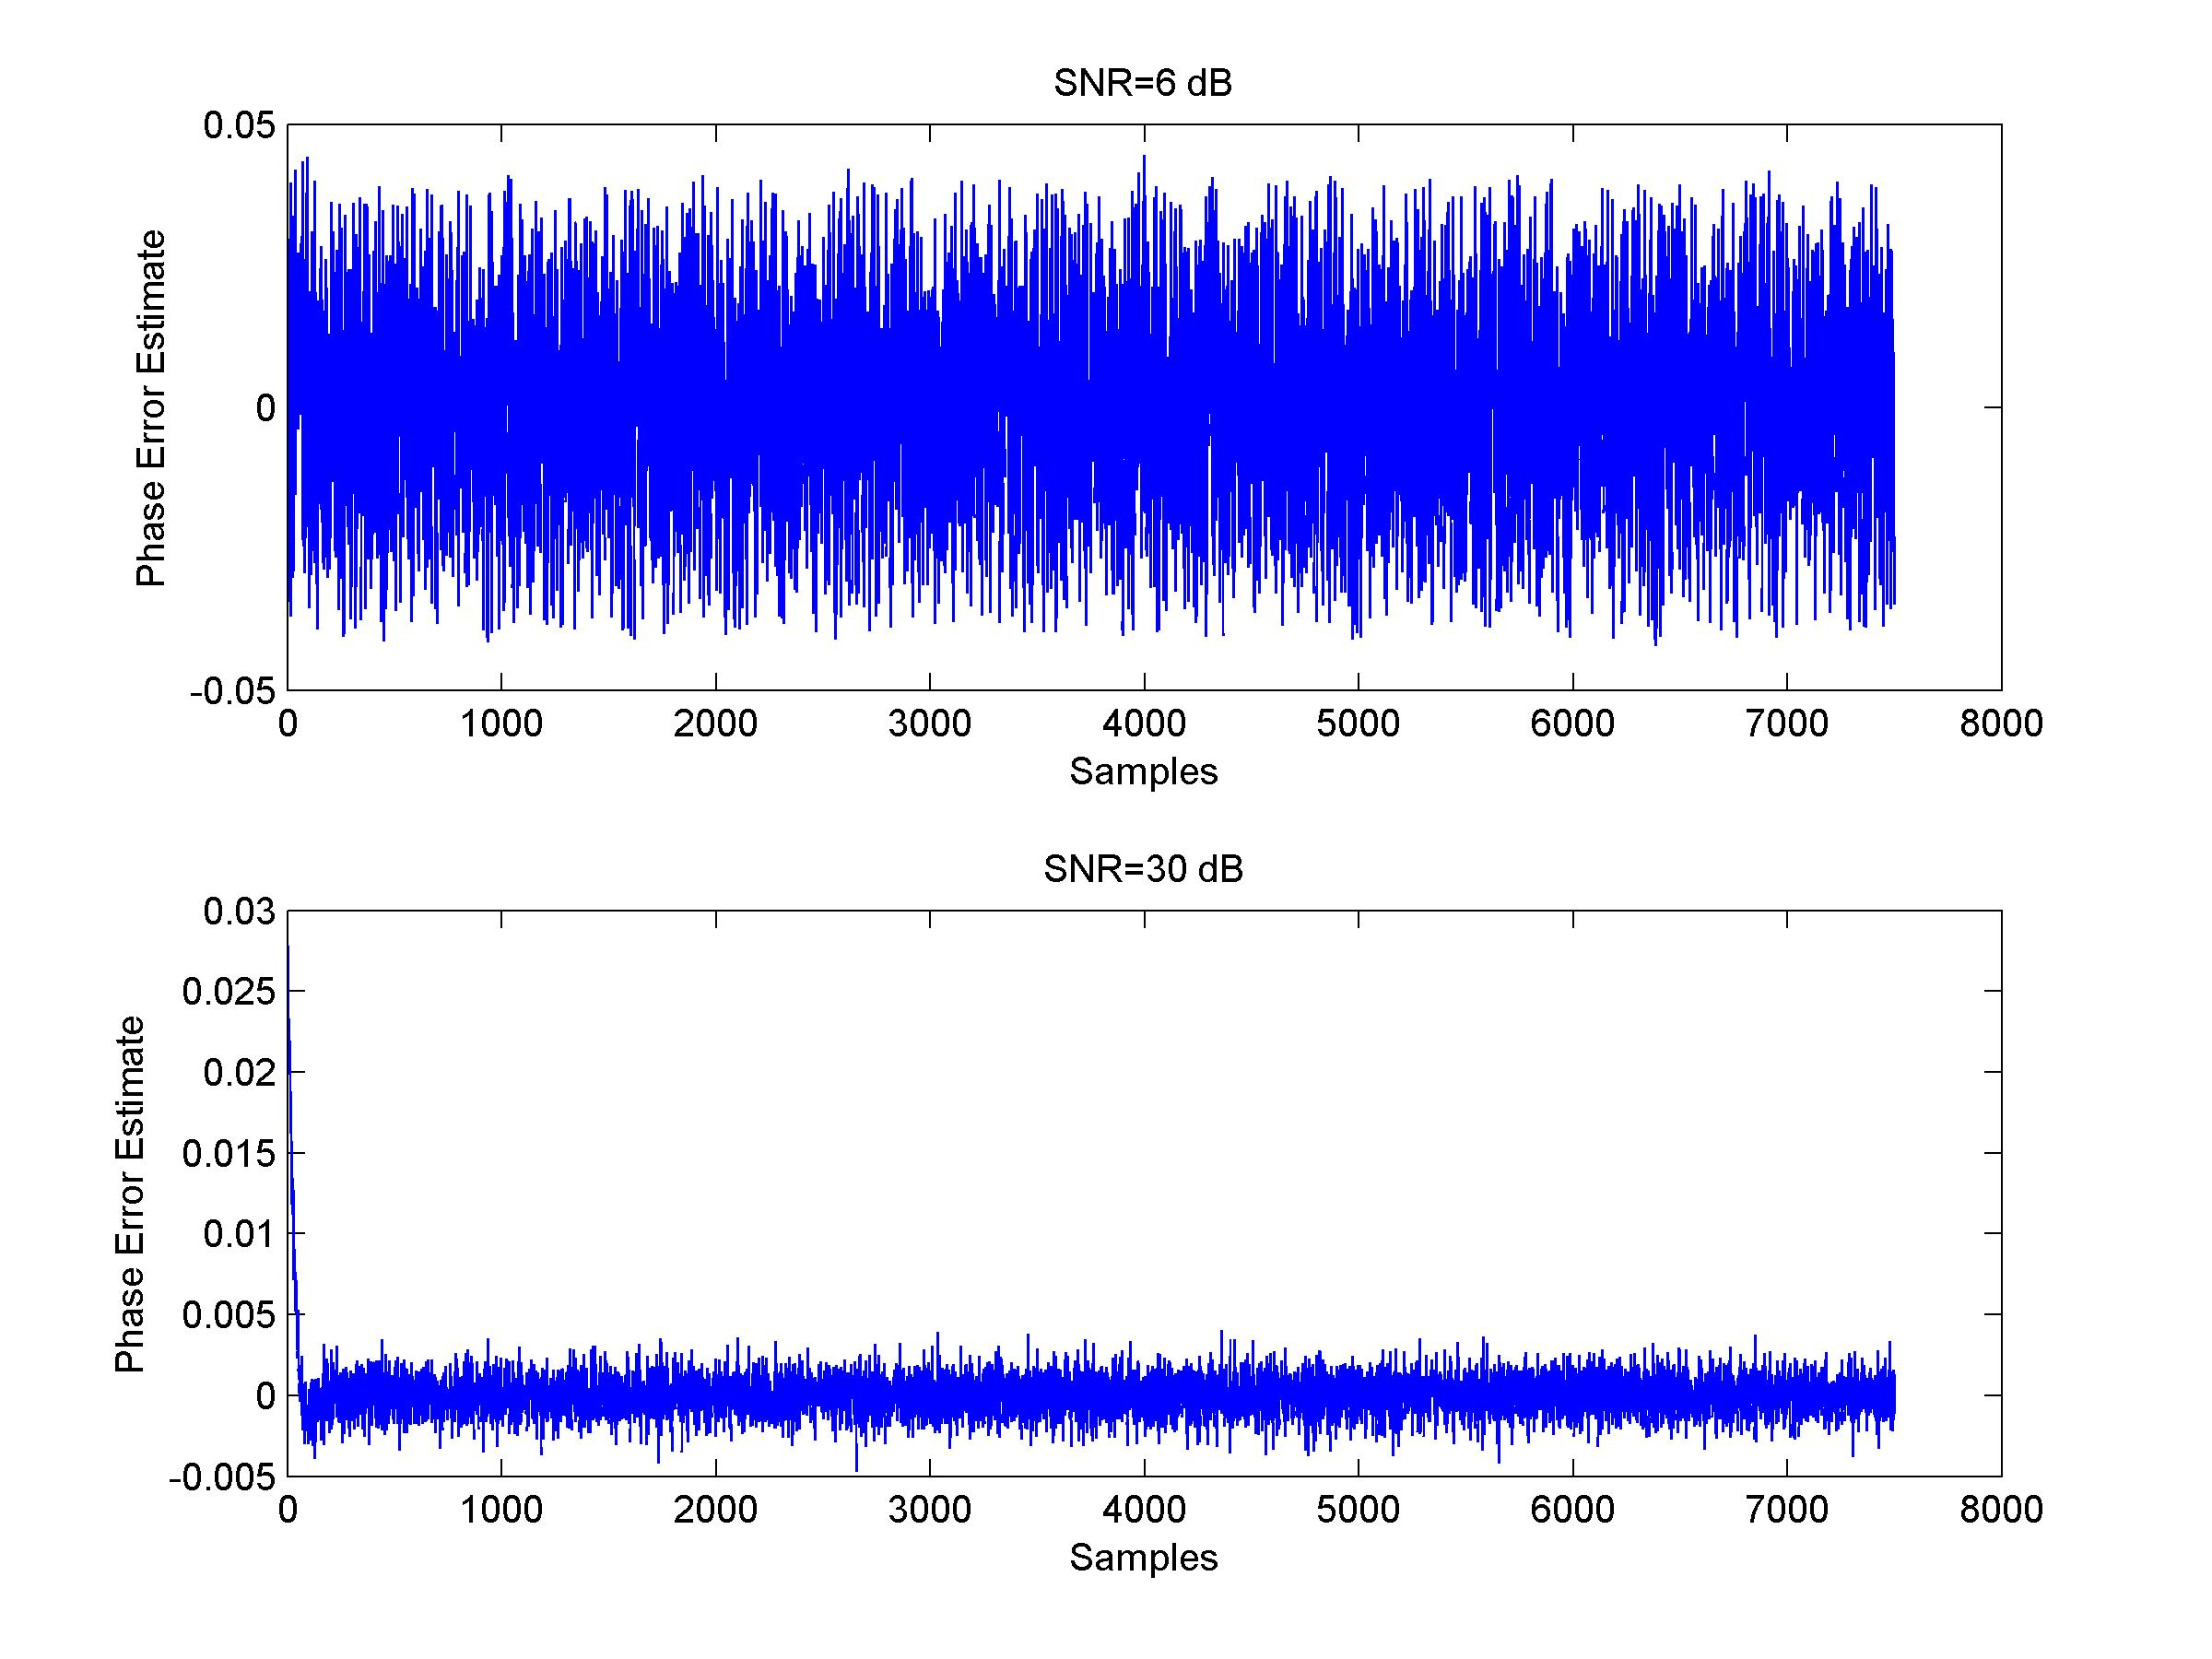
\includegraphics[width=0.7\textwidth]{qpLoopFilterpo_ddr1.jpg}
%\caption{The loop filter output of the Decision Directed Recovery Loop for an input signal with 30 degrees phase offset \label{fig:ddrTransphase}}
%\end{figure}
%
%
%\subsubsection{Constellation Plots  for Phase Recovery}
%\begin{figure}[H]
%\centering
%\hspace*{-2cm}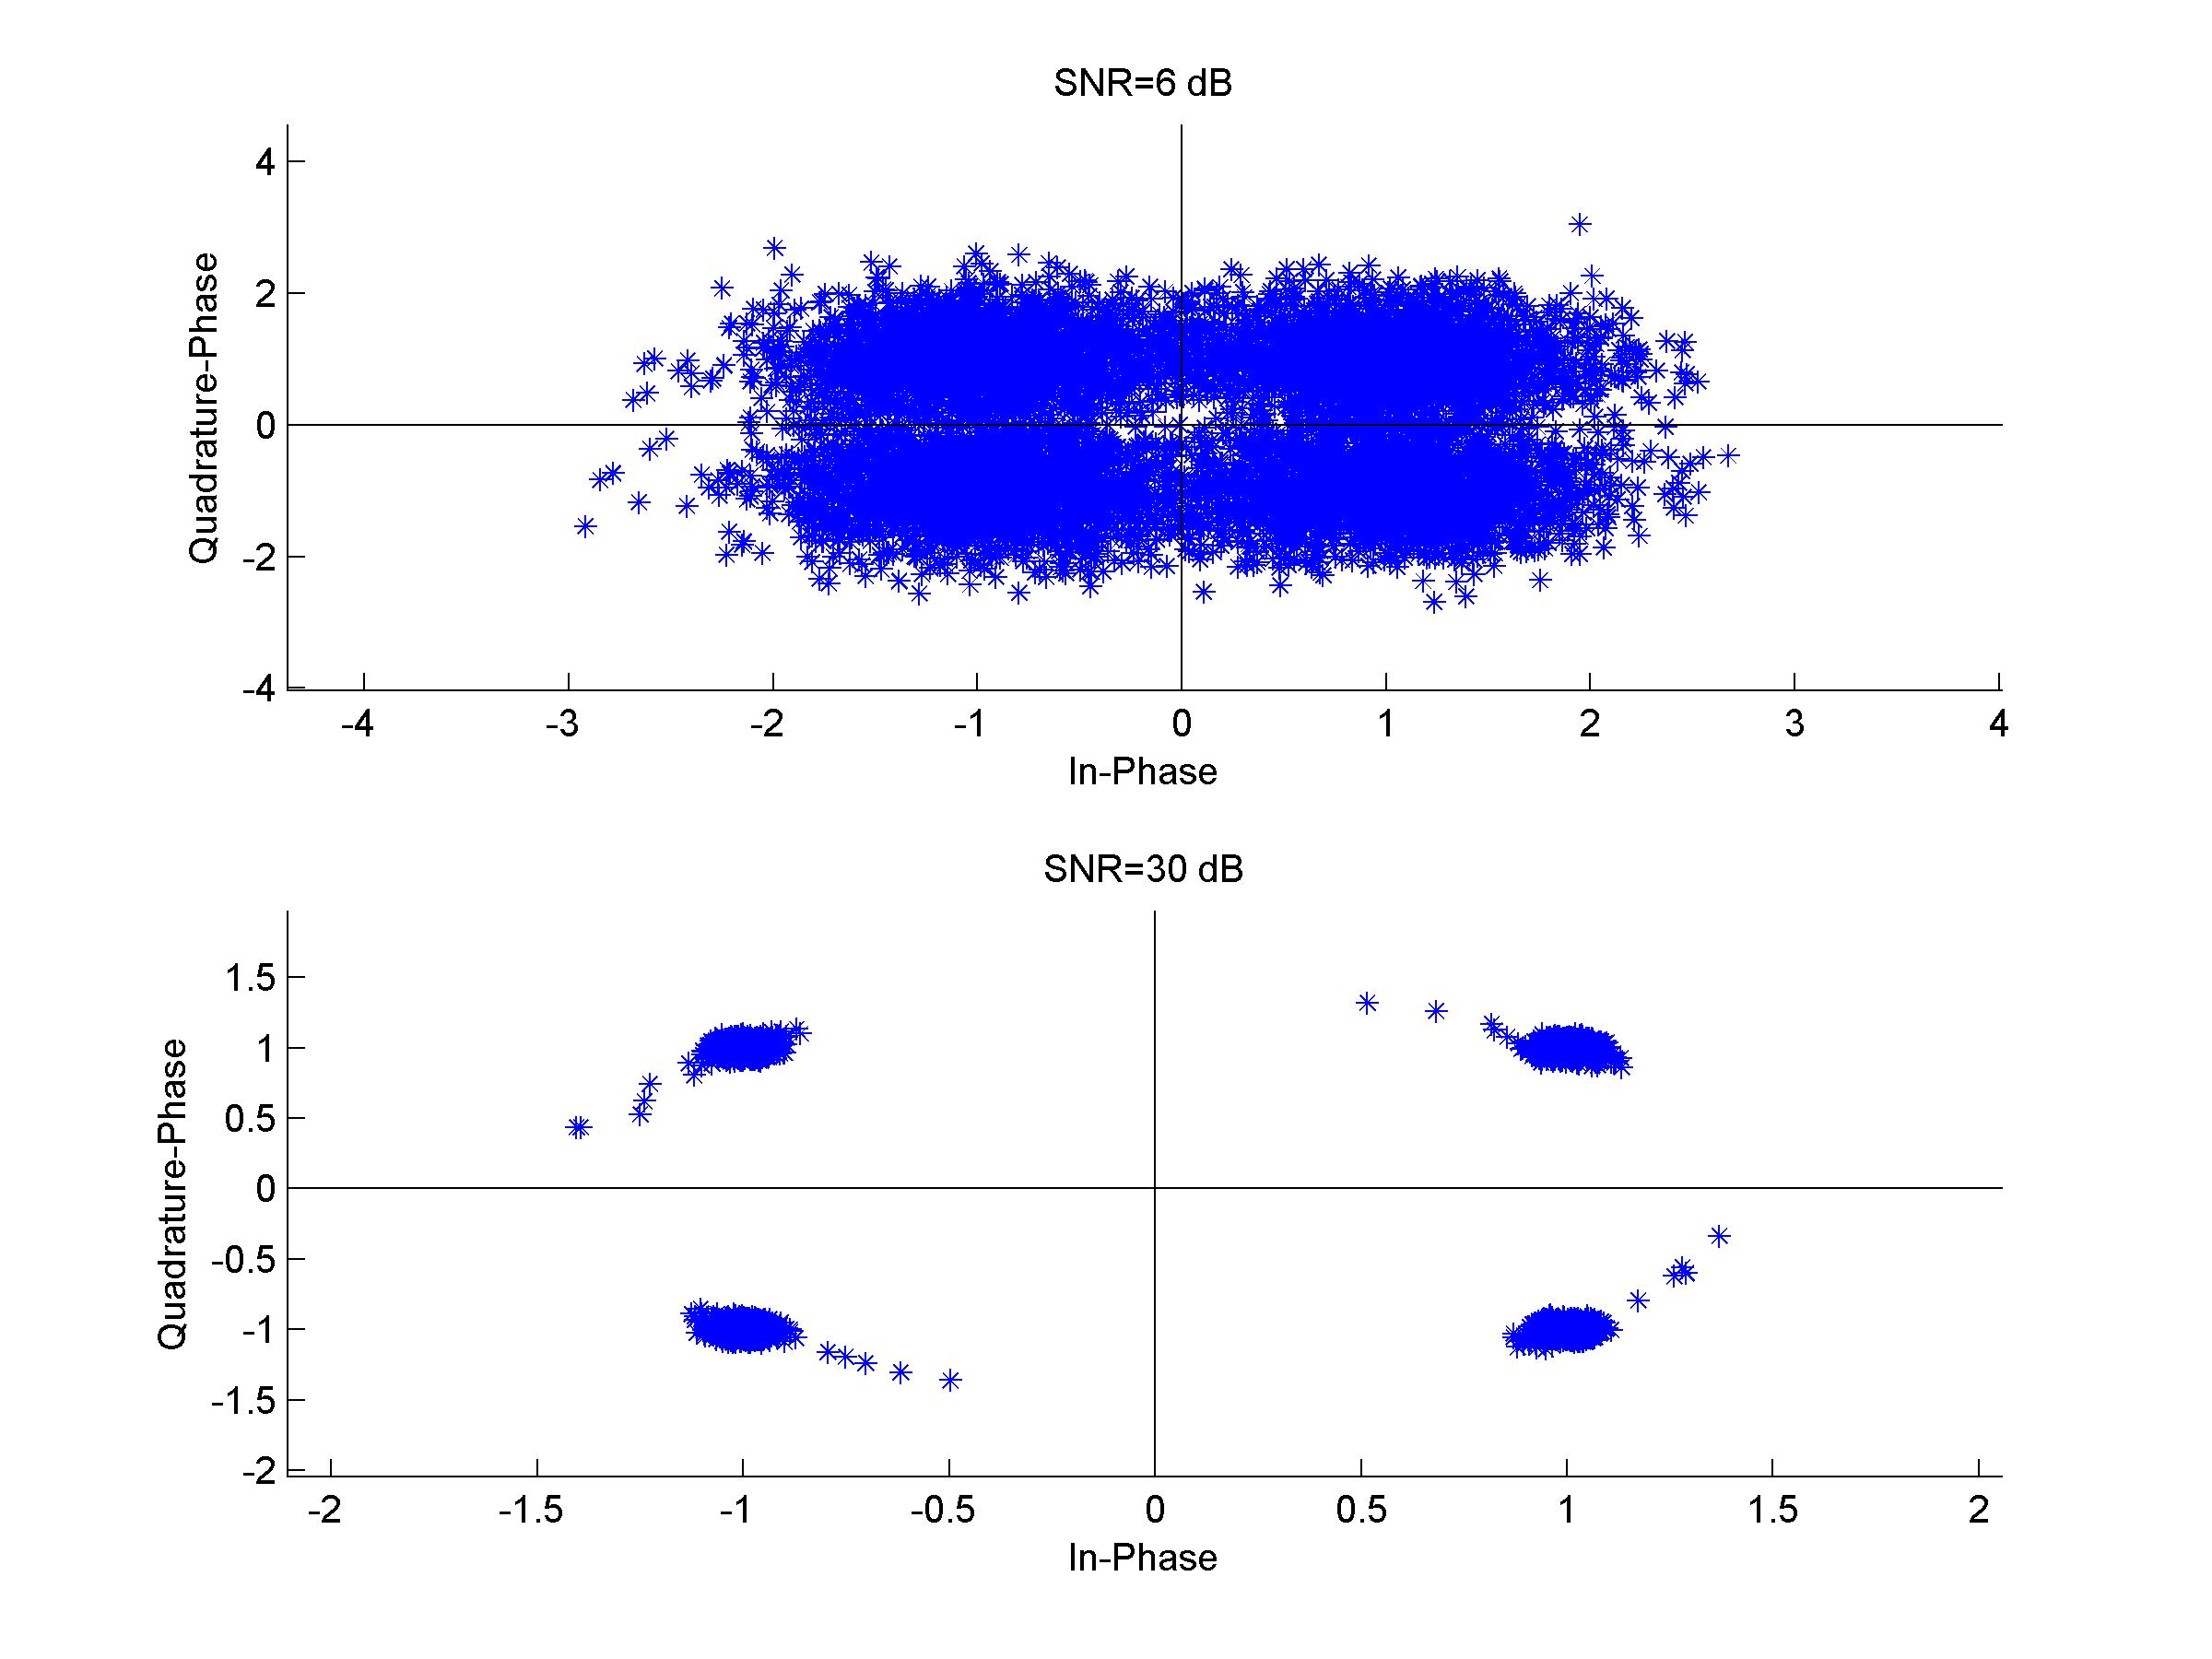
\includegraphics[width=0.7\textwidth]{qpConstpo_ddr1.jpg}
%\caption{The resulting constellation plot of the output of the system with Decision Directed Recovery Loop for an input with 30 degrees phase offset at 6dB and 30dB SNR \label{fig:ddrConstPhase}}
%\end{figure}
%
%\subsubsection{BER Plots for Phase Recovery}
%\begin{figure}[H]
%\centering
%\hspace*{-2cm}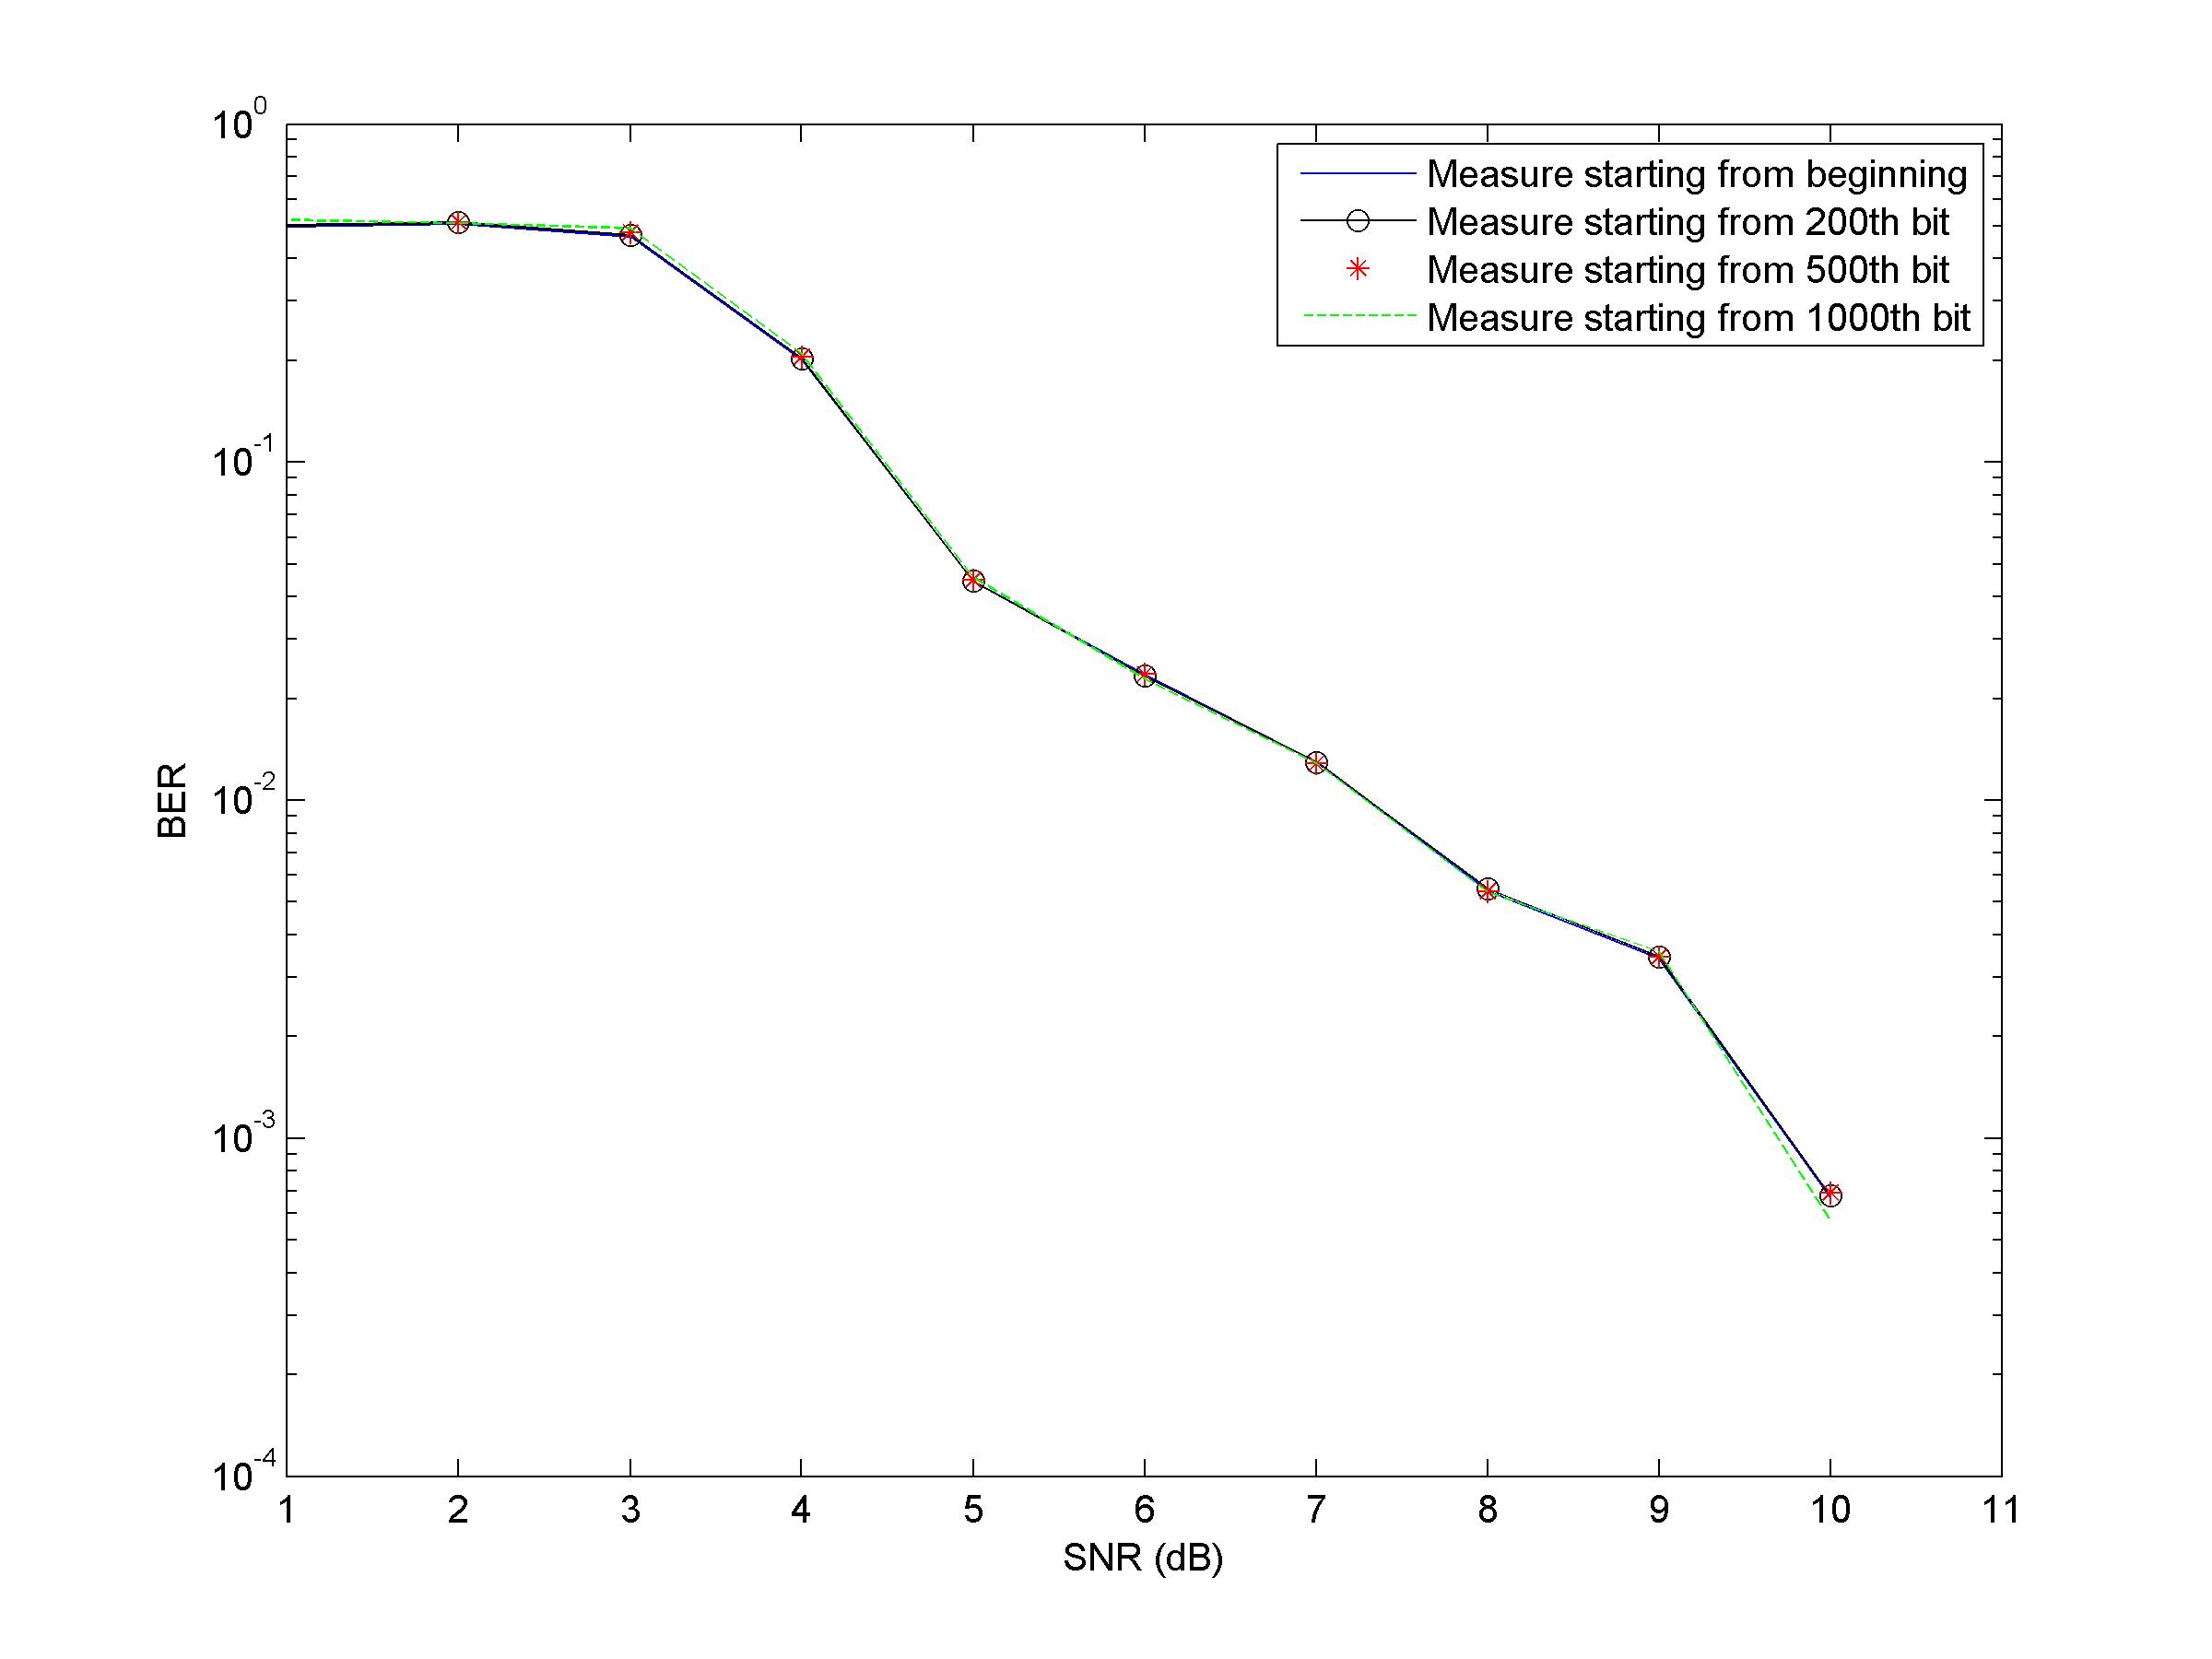
\includegraphics[width=0.7\textwidth]{qpBERpo_ddr1.jpg}
%\caption{BER plots of the system with Decision Directed Recovery Loop for an input with 30 degrees phase offset (using output bits starting from different indexes) \label{fig:ddrBERphase}}
%\end{figure}
%
%\subsubsection{BER Plots for Carrier Recovery}
%\begin{figure}[H]
%\centering
%\hspace*{-2cm}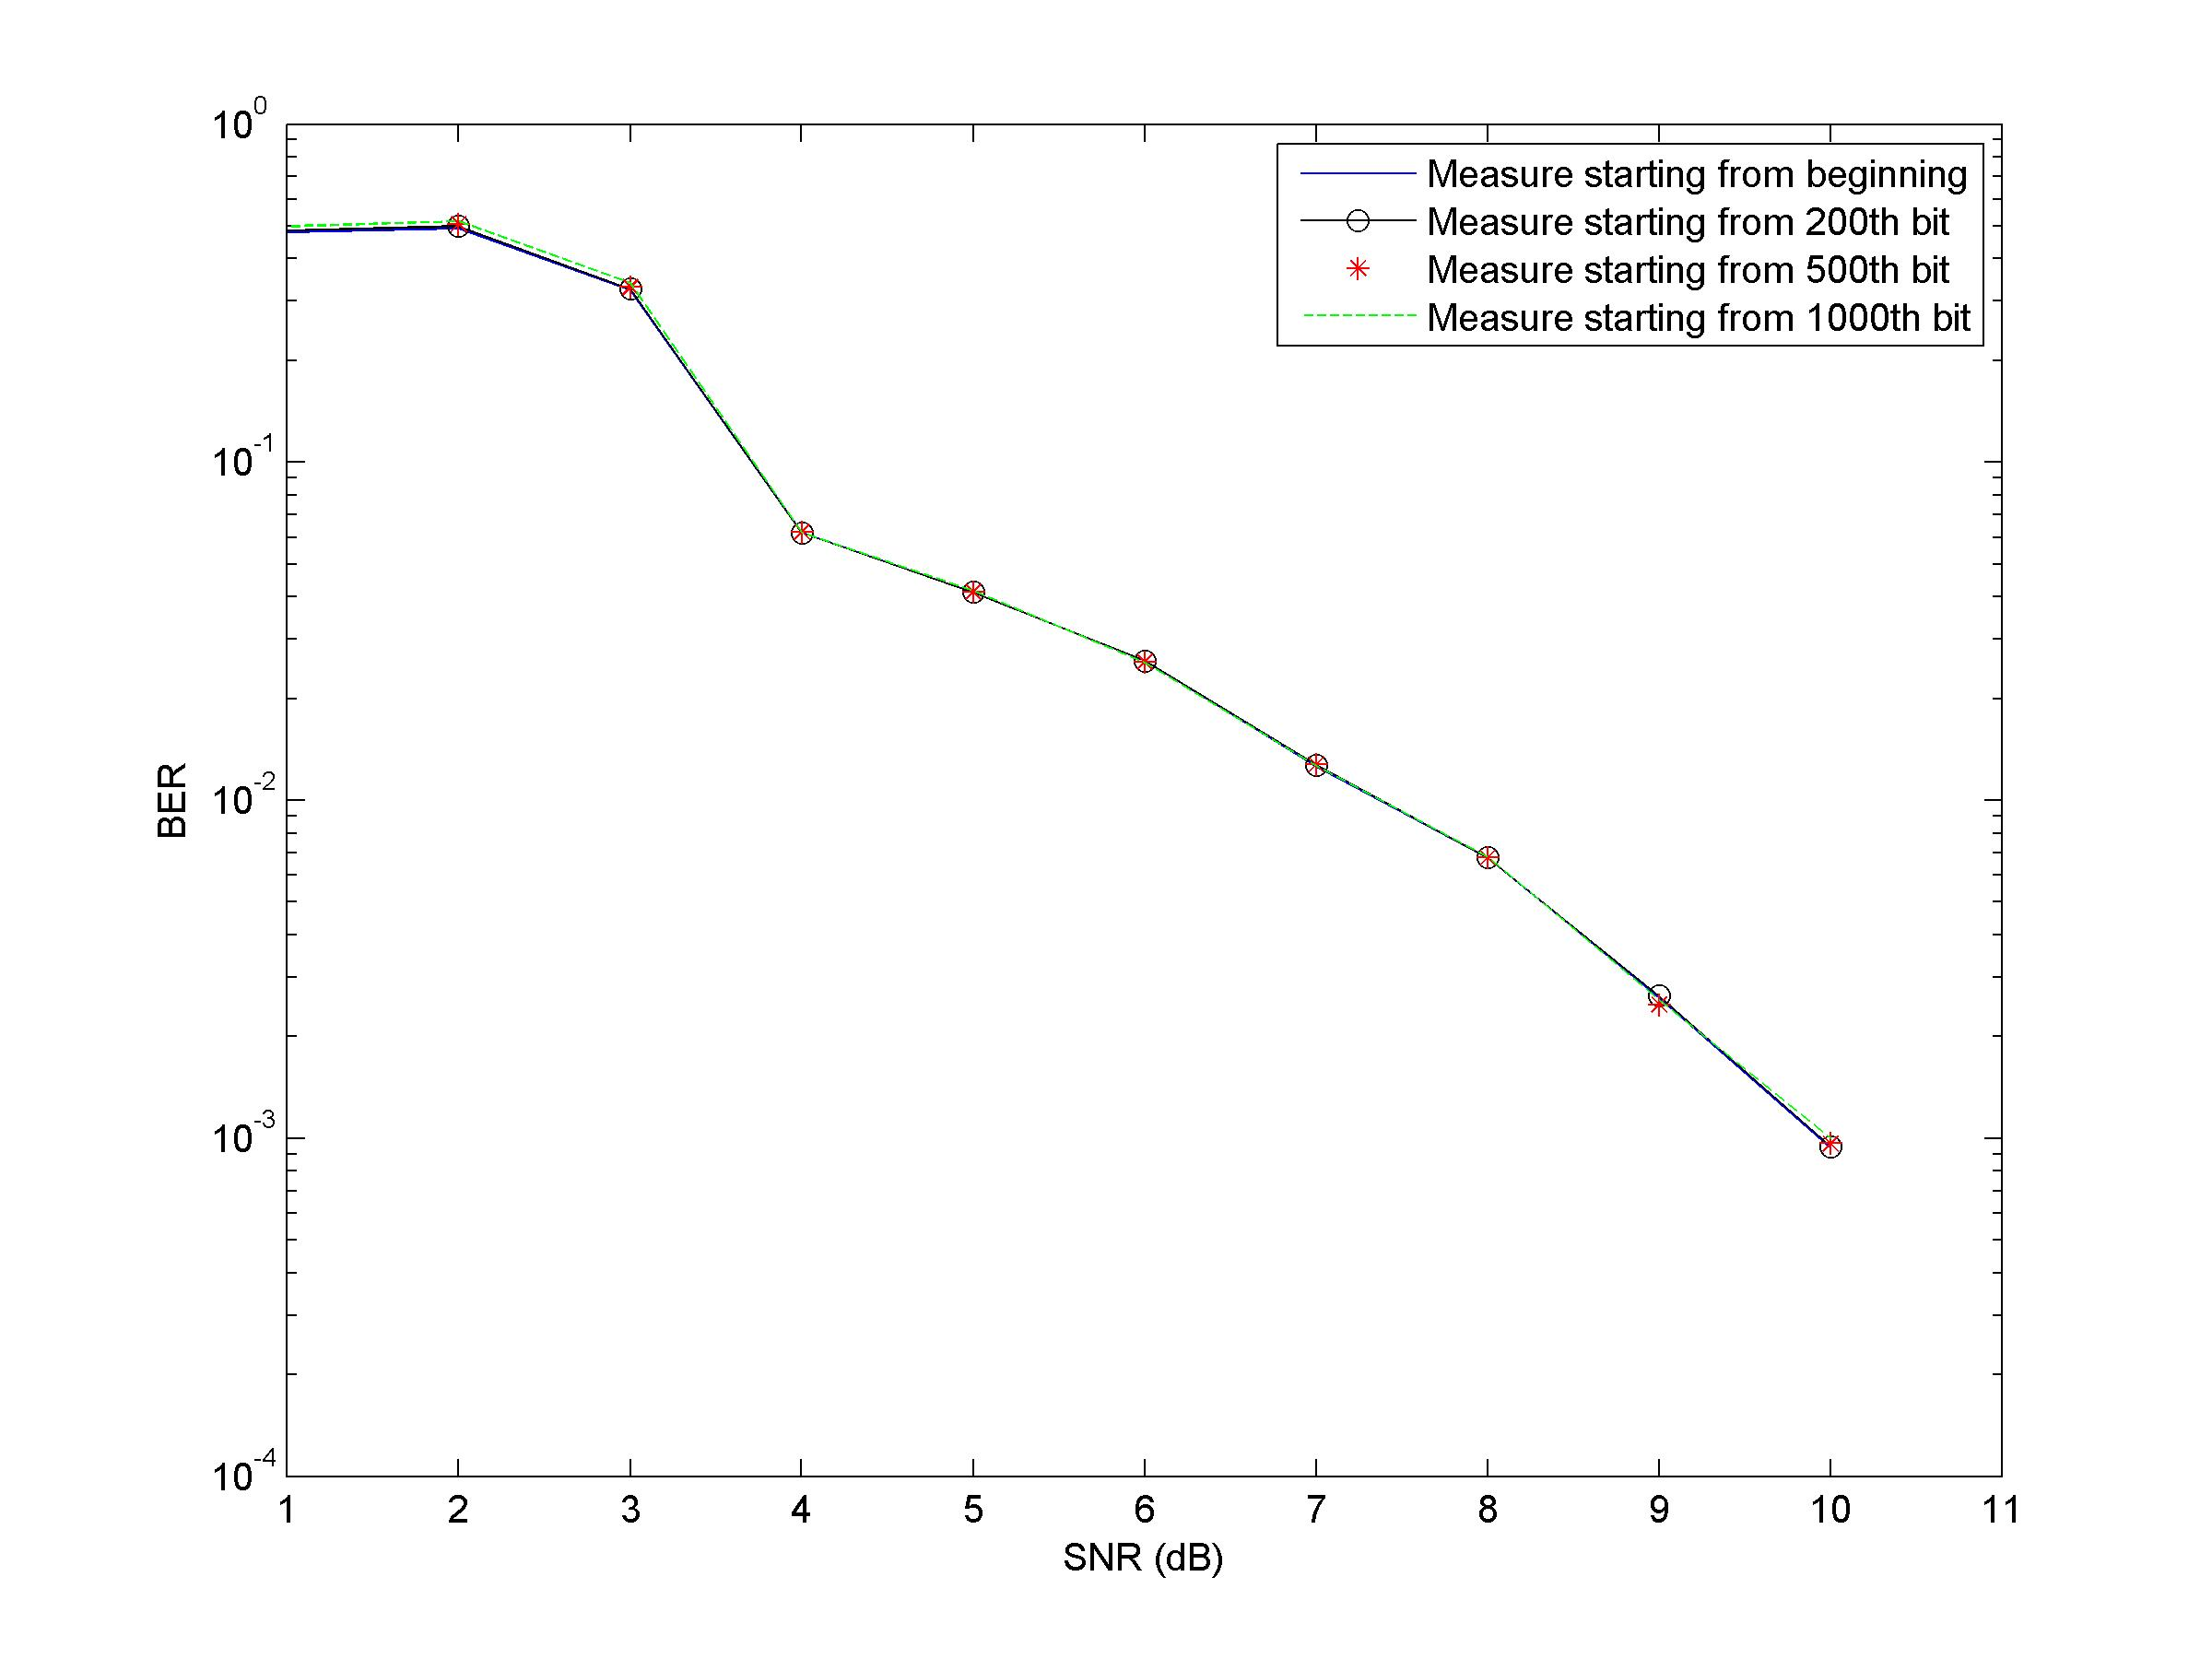
\includegraphics[width=0.7\textwidth]{qpBERfo_ddr1.jpg}
%\caption{BER plots of the system with Decision Directed Recovery Loop for an input with 1ppm frequency offset (using output bits starting from different indexes) \label{fig:ddrBERFreq1}}
%\end{figure}


\newpage
\section{Conclusion}
\label{sec:conc}

The objective of this step was to recover the system from the phase and frequency offsets that might be present in the received signal. To handle the noncoherent error introduced into the system, feedback loops (Costas and Decision Directed) were installed. These use control feedback to track out the errors by first finding a metric for the error, then using integrators to track away that error. 

The `S' Curve results for the Costas type setup give indication of how the system reacts to different degree phase and frequency error.  Notice, in each of the graphs [\ref{fig:costasSphase}, \ref{fig:costasSfreq}], the estimation error is periodic.  This is because the the metric does a good job approximating for phase at small phase levels, but of course has some error.  We see the same results in the Decision Directed cases as well [\ref{fig:ddrsphase}, \ref{fig:ddrsfreq}].

In the transience plots, notice that the error in the 6 dB is zero mean and has magnitude around .01.  The 30 dB plot [\ref{fig:costasTransPhase}]  shows the typical convergence shape we would expect.  We feel that the same structure exists in the lower SNR case, but the settling time happens in only a few samples and gets lost.  This pattern is repeated for the frequency estimation trials as well [\ref{fig:costasTransFreq1}, \ref{fig:costasTransFreq2}].  Again, the Decision Directed loops have the same form [\ref{fig:ddrTransphase}, \ref{fig:ddrtransFreq1}, \ref{fig:ddrTransFreq2}].

The constellation plots are also informative.  Note how in the Phase Costas Loop, Figure~\ref{fig:costasConstPhase}, there are a few points that have the stretching characteristic of phase error.  Then the blurring stops and the loop locks on, creating the clumps for the symbols.  This same tracking happens in the Decision Directed constellation [\ref{fig:ddrConstPhase}].  The frequency offsets never show this tracking, perhaps because they get locked on so quickly the tail never appears.

Looking at the loop filter output results for the system where a phase offset is introduced, it can be seen that phase error estimate converges to zero very fast. This means that we don't really need to throw any of the received bits. This result can also be deduced from the BER graphs provided in the results section. When a phase offset is introduced, dropping bits doesn't really change the resulting probability of error of the system. Thus we can conclude that if the phase error estimate converges fast enough dropping bits doesn't really affect the efficiency of the system in term of bit error rate. 

The same results are valid for the system with frequency offset too, as the frequency error estimate reaches the steady-state fast enough that dropping bits doesn't really change the bit error rate of the system. 

\appendix
\newpage
\bibliographystyle{plain}
\bibliography{step4}
\newpage
%% the \\ insures the section title is centered below the phrase: Appendix B
%\section{Project Assignment}
%\label{app:assign}
%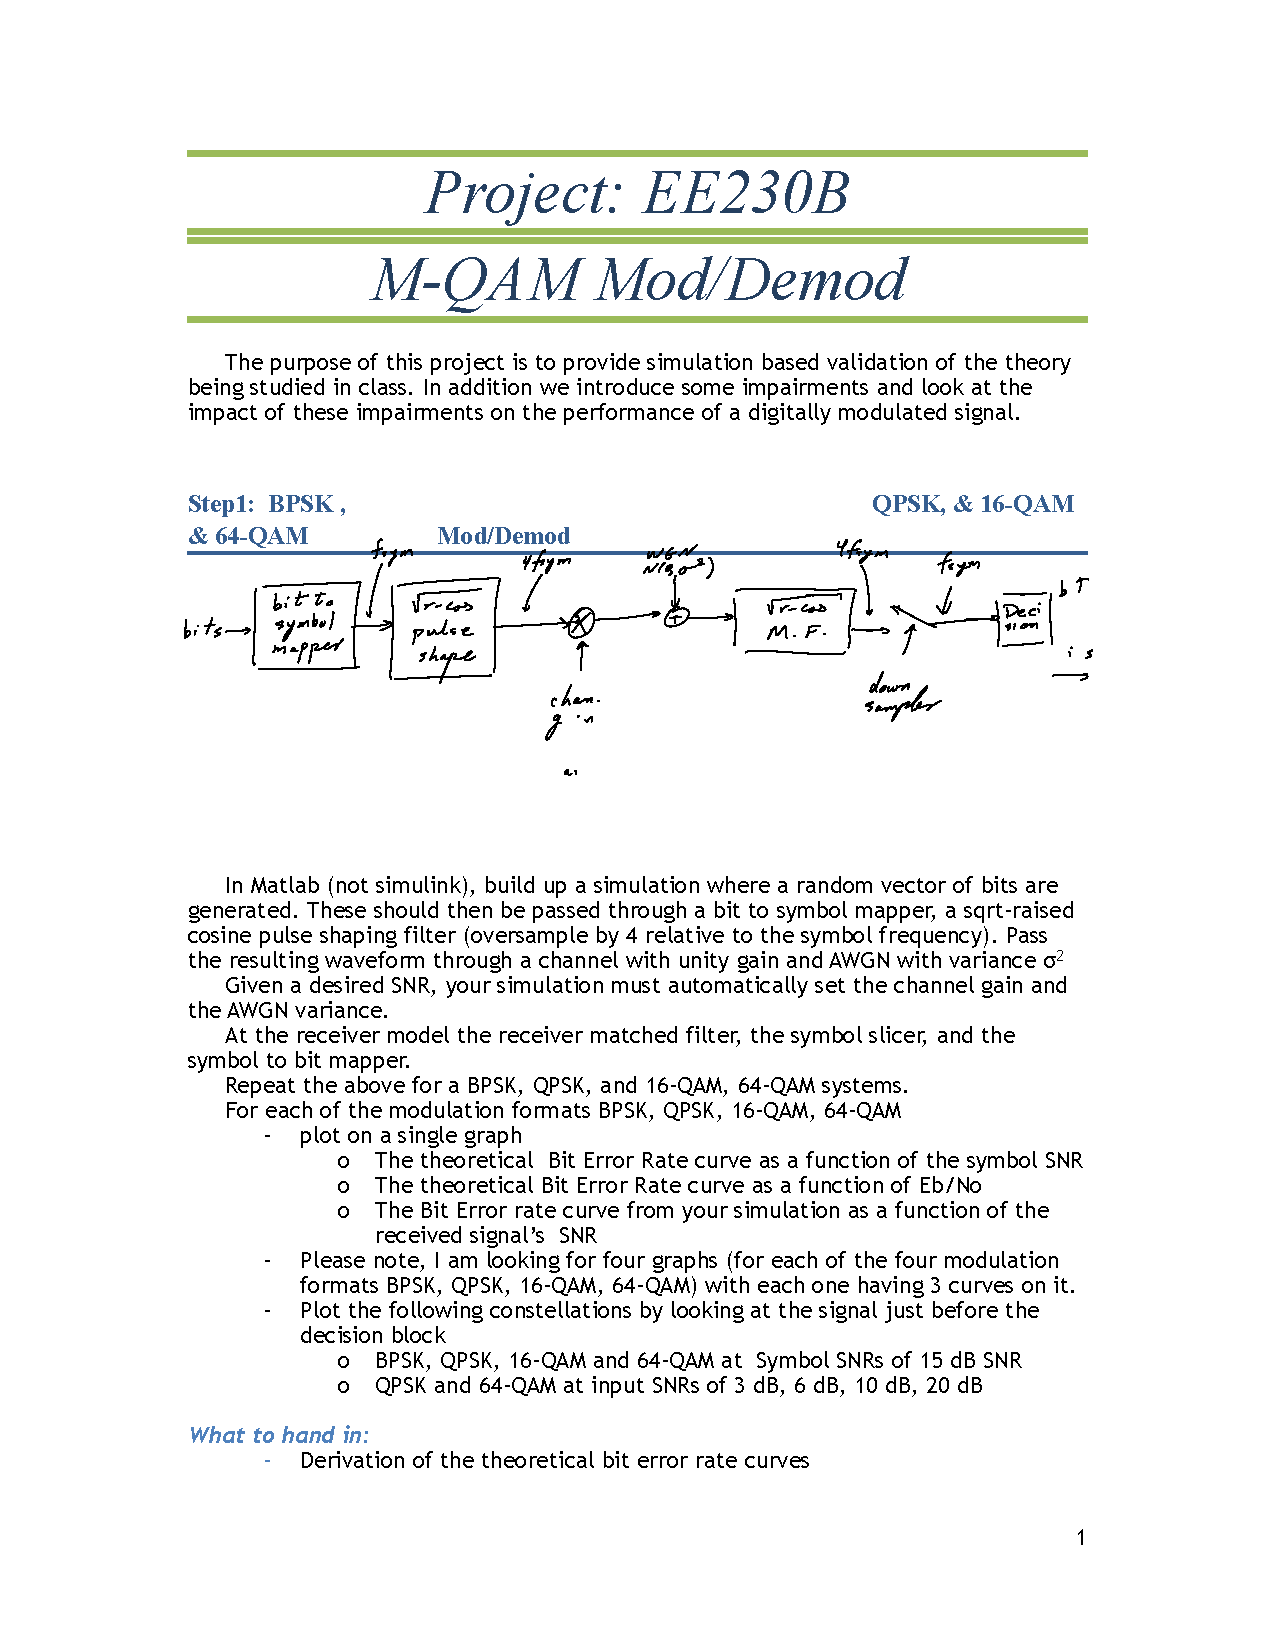
\includepdf[pages={1-5}]{project_overview.pdf}
%\cleardoublepage
%\newpage

\section{Random Bit Sequence Generator}
\label{app:random_bit_generator}
\lstinputlisting{random_bit_generator.m}

\section{Bit to Symbol Mapper}
\label{app:bittosym}

\subsection{QPSK Modulation}
\label{app:qpsk_mod}
\lstinputlisting{qpsk_mod.m}

\section{Square Root Raised Cosine Filter}
\label{app:sqrt_raised_cosine}
\lstinputlisting{sqrt_raised_cosine.m}

\section{Up Sampler}
\label{app:impulse_train}
\lstinputlisting{impulse_train.m}

\section{Additive Gaussian White Noise Channel}
\label{app:awgn_channel}
\lstinputlisting{awgn_complex_channel.m}

\section{Sampler}
\label{app:sampler}
\lstinputlisting{sampler.m}

\section{Decision Block}
\label{app:dblocks}
\subsection{QPSK Demodulation}
\label{app:qpsk_demod}
\lstinputlisting{qpsk_demod.m}


\end{document}